\subsection{MIR Instructions}

SableWasm MIR uses control-flow-graph (CFG) based representations in static-single-assignment (SSA) form to represent code body in function definitions. We have provided an introduction to CFG and SSA in the background chapter. Here is a quick recap. CFG splits the control flow within the function into basic blocks. A basic block represents the most extended instruction sequence without control flow transfer, such as branching. Note that for function calls, we take a similar approach that LLVM adopted. We will come back to this in detail later in the section. Additionally, SSA requires that all values must have a unique definition site. Hence, in SSA form, the use-def chain is trivial to compute, while in a traditional CFG, one would need to extract from the graph with the help of reaching definition analysis. SableWasm instruction set is similar to WebAssembly bytecode in terms of semantics for most of the instructions. However, it operates over an infinite register machine instead of a stack-based machine. We also want to keep the size of the SableWasm instruction minimal. Hence, some of the instruction has different semantics compared to the counterpart appears in the WebAssembly specification. In this section, we will cover the design and implementation of SableWasm instructions. The following section will cover the translation strategy between WebAssembly bytecode and the SableWasm instruction set and instruction reduction rules.  Figure~\ref{fig:sablewasm-mir-inst} provides a general illustration of the design of the SableWasm instruction set. The SableWasm instruction sets can currently cover all the instructions set defined in WebAssembly specification, along with several extensions such as multivalue and SIMD vector operations.

\begin{figure}
  \centering
  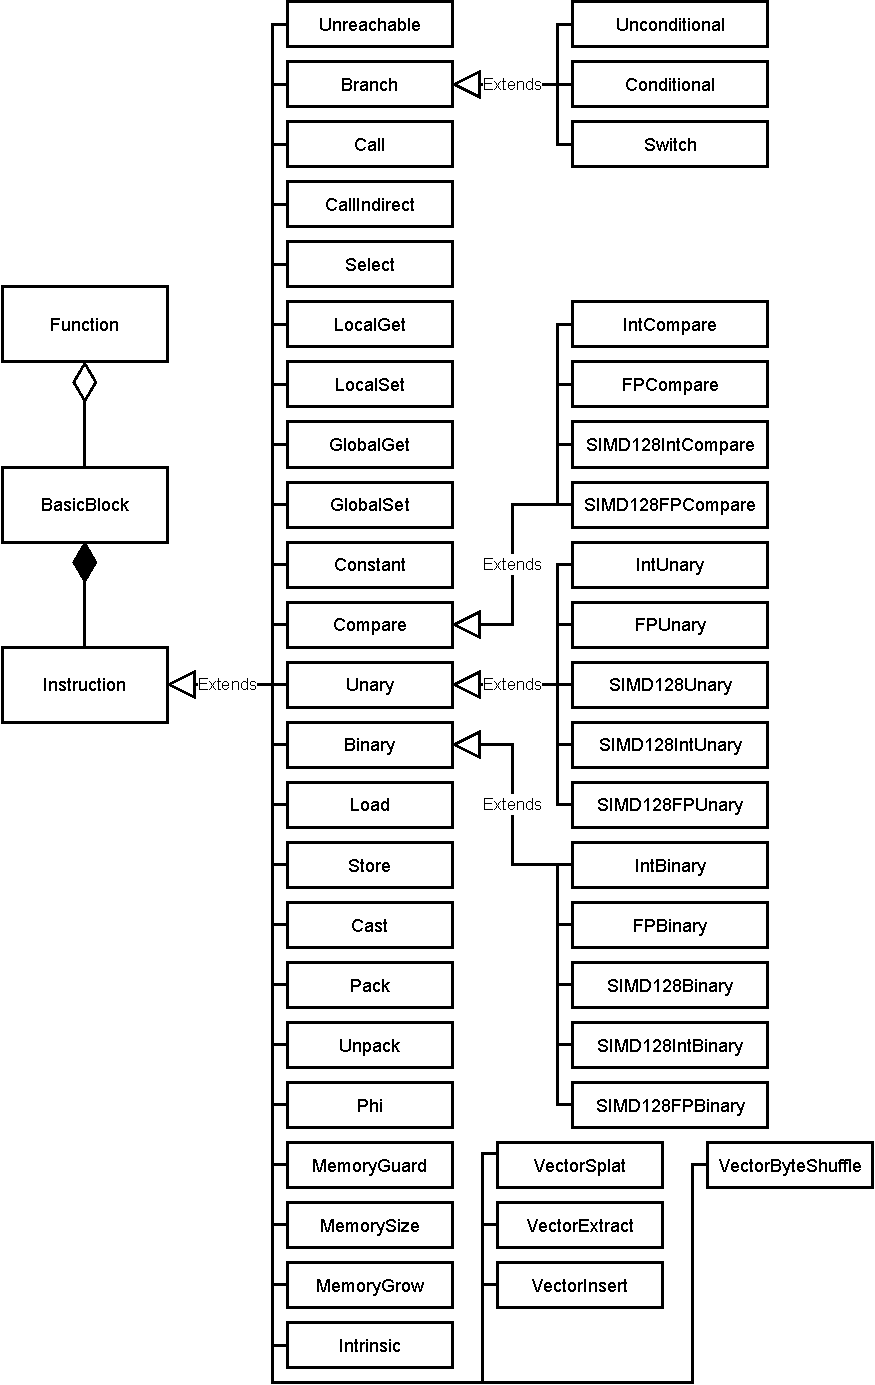
\includegraphics[width=0.85\textwidth]{Images/4.MIR/sablewasm-instruction.pdf}
  \caption{SableWasm MIR Instructions}
  \label{fig:sablewasm-mir-inst}
\end{figure}

\paragraph{Terminating instructions} As we discussed above, SableWasm split the function control flow into basic blocks, which contain the maximum amount of consecutive instructions without control flow transfer. In addition, SableWasm, similar to many other SSA form instruction sets, defines a particular group of instructions called terminating instructions. These instructions signal a control flow transfer out of the current basic block, and they must only appear as the last instruction in any given basic block. SableWasm defines four different terminating instructions: unreachable, unconditional branching, conditional branching and table branching. If the control flow reaches a \texttt{unreachable} instruction, the runtime system will signal a runtime panic. The \texttt{unreachable} instruction in SableWasm is identical to its counterpart in WebAssembly in terms of semantics. The \texttt{Unconditonal} instruction is an unconditional control flow transfer, as the name suggests. It refers to a basic block as the operand. At runtime, the instruction will always transfer the control flow to the target basic block. \texttt{Unconditional} is similar to the \texttt{br} instruction defined in WebAssembly specification. On the other hand, \texttt{Conditional} is a conditional branching. It takes a value and two basic blocks as its operands. At runtime, the instruction will compare the value against integral value zero. If the value equals zero, the instruction will transfer the control flow to the `false' basic block, otherwise, to the `true' basic block. SableWasm's \texttt{Conditional} instruction is similar to \texttt{br.cond} defined in WebAssembly. The last terminating defined in SableWasm is \texttt{Switch}. \texttt{Switch} instruction is comparable to the \texttt{br.table} instruction in WebAssembly. The instruction takes a value, a list of basic blocks, and a default branching basic block as its operands. At runtime, \texttt{Switch} will interpret the value as an integral value and dispatch accordingly. If the value is within the branching list's range, it will redirect the control flow to the basic block referred to by the index. Otherwise, \texttt{Switch} will transfer the control flow to the default basic block.

\paragraph{Function call} In SableWasm, we provide two instructions for function calls defined in WebAssembly specification, direct function calls and indirect function calls. \texttt{Call} defines a direct function call where the callee is known at compile time. It takes a function as callee and a list of arguments as operands. On the other hand, \texttt{CallIndirect} defines an indirect function call. It implements the indirect function call protocol defined in WebAssembly specification. A quick reminder, in WebAssembly, an indirect function call takes an indirect table, the table index, the expecting function type and a list of values as arguments. At runtime, the system should first check if the index is valid for the indirect table and fetch the function pointer and its actual signature accordingly. Then, the system should compare the signature against the expecting type. If the signature matches the type, the runtime system will transfer the control flow to the function referred to by the function pointer. Implementing the signature verification mechanism is backend-specific; we will return to this topic in the next chapter. Note that we do not treat function call instructions as terminating instructions, even transferring the control flow to other locations. In SableWasm MIR, we follow the design that appeared in LLVM intermediate representation. It is guaranteed that the control flow will continue to the next instruction for function call instructions. Hence, from the basic block's local point of view, their control flow is pre-determined, and there is no difference compared to other non-terminating instructions.

\paragraph{Local and global variable access} In WebAssembly, instructions have access to locals defined by its parent function and global variables defined by its enclosing module. SableWasm defines getter and setter instruction for both local and global variables to implement the specification. Their semantics are the same compare to WebAssembly's counterparts. We will skip the detail here, but one can consult the WebAssembly specification for detailed information.

\paragraph{Numerical operations} In SableWasm, we classify the numerical operations into three different categories, the \texttt{Compare} instructions, \texttt{Unary} instructions, and \texttt{Binary} instructions. The \texttt{Compare} instructions implements the comparison between values, such as `equal to'. They always yield a 32-bit integer as WebAssembly specification suggests. The \texttt{Unary} and \texttt{Binary} implements , as their name suggests, unary and binary operations between values. The result of \texttt{Unary} and \texttt{Binary} instruction is dependent on the opcode. On the other hand, we can also orthogonally classify the instructions into integer, floating-point and packed integer and packed floating numbers. Note that in MVP WebAssembly, there are only integer and floating-point value operations; the SIMD operation extension proposal adds the packed value operation to the instruction set. In the WebAssembly SIMD extension proposal, the vector value does not store its shape information in the types. Instead, the packed value instructions' opcodes keep track of the shape of the vector values, which leads to the blot of instruction opcodes. In SableWasm, we separate the instruction opcode from the vector shape. For each of the packed value operations, it must have either a \texttt{SIMD128IntLaneInfo} or \texttt{SIMD128FPLaneInfo}. Figure~\ref{fig:sablewasm-mir-inst} shows all the class of numerical operations defined in SableWasm. For detailed opcode of each numerical instruction class, we include them in the thesis appendix.

\paragraph{Load and store} \texttt{Load} and \texttt{Store} instruction provides access to the linear memory for SableWasm MIR. Although in the current version of WebAssembly, the module can contain at most one linear memory. All load and store implicitly refer to this linear memory \footnote{This subject to change in the future version of WebAssembly.}. \texttt{Load} instruction takes a linear memory and an integer value as operands. At runtime, the value will treat as the address (or offset) respective to the start of the linear memory, and the instruction yields to fetched result. In WebAssembly, the \texttt{load} instruction associates with a type and an extension method. For example, \texttt{i32.load8\_s} load an 8-bit integer from the linear memory, and then signed extends the fetched byte into a 32-bit integer. In SableWasm, \texttt{Load} instruction only associates to an integer value, namely the load width. The load width must equal to or smaller than the load type's width. Also, SableWasm \texttt{Load} always perform zero-extension on loaded value. Hence, when translating WebAssembly's sign-extended load into SableWasm's \texttt{Load}, one must combine the load instruction with a cast instruction. We will come back to this later in the chapter. \texttt{Store} instruction also associate with a store width. Like the load width defined for \texttt{Load} instruction, store width must also be equal to smaller than the store value type's width. At runtime, the system will first perform bit truncate to the value and then store the result into the linear memory. One may notice that in SableWasm, we erase the alignment attribute and offset attribute defined in WebAssembly. Currently, we do not support alignment hints from the WebAssembly module. In SableWasm, the load and store always have the alignment requirement of one byte. This implies that the load and store can happen anywhere in the linear memory, which corresponds to WebAssembly's linear memory specification.

\paragraph{Linear memory manipulation} WebAsseembly specification defines three instruction can manipulate linear memories, such as \texttt{memory.size}, \texttt{memory.grow}. Like the \texttt{load} instruction we covered in the previous paragraph, all these instructions operate over the implicitly defined unique linear memory within the module. In SableWasm, we provide similar \texttt{MemoryGrow} and \texttt{MemorySize} instruction. The semantics of the SableWasm's memory manipulation instruction is the same as their WebAssembly counterparts, except that the linear memory needs to be explicitly stated. In SableWasm, we introduce a special instruction, \texttt{MemoryGuard} which is an explicit memory boundary check. In WebAssembly, all \texttt{load} and \texttt{store} instruction need to check for linear memory out of bound error before access. SableWasm separates the bound check from the memory access. One advantage of this is that one may implement static memory bounds check elimination optimization over SableWasm MIR. Additionally, one backend may provide different strategies for handling boundary checks, such as utilizing invalid virtual memory pages with the operating system's help. In this case, we only need to modify the translation pattern for \texttt{MemoryGuard}. \texttt{MemoryGuard} takes a linear memory and an integer value as the operand. It also associates with an integer immediate, known as guard width. At runtime, the system will perform a boundary check over the linear memory starting from the given address to determine if it contains at least a given number of bytes ahead. If there are not enough bytes available, the system should signal a runtime panic.

\paragraph{Pack and Unpack} WebAssembly multivalue specification \footnote{WebAssembly Multi-value Proposal: \url{https://github.com/WebAssembly/multi-value}} relaxes the constrains on the function type. Functions now can return multiple values instead of at most one value. To support these features, we introduce \texttt{Pack} and \texttt{Unpack} instructions, along with extending WebAssembly's type system. \texttt{Pack} instructions group multiple values into an ordered tuple, while the \texttt{Unpack} reverse the operation by retrieving the value from tuples by index. In the case where a function returns multiple values, we use a tuple instead. SableWasm treats tuples as a first-class values; however, currently, tuples cannot be recursive. We will come back to this later in the chapter when we visit the type systems of SableWasm MIR. The index of the \texttt{Unpack} must be an immediate value in the current version of SableWasm MIR and is verified at compile time.

\paragraph{Vector operations} In the previous paragraph, we introduce the numeric operations defined in SableWasm MIR. However, several instructions does not fix into neither \texttt{Unary} nor \texttt{Binary} instructions. Hence, to faithfully support the SIMD operations introduced by the extension proposal, we add four vector-specific operations into SableWasm MIR. They are \texttt{VectorSplat}, \texttt{VectorExtract}, \texttt{VectorInsert} and \texttt{VectorByteShuffle}. \texttt{VectorSplat} will broadcast the operand value to all lanes in the result vector. SableWasm MIR defines vector splat operation for both packed integer vector and packed floating-point vector. \texttt{VectorExtract} is similar to the \texttt{extractelement} defined in LLVM intermediate representation. It takes a vector as the operand and also associates itself with an immediate integer value. At runtime, the system extracts the value of the given lane and yields as a result. \texttt{VectorInsert} is similar to \texttt{insertelement} defined in LLVM. It will replace the vector operand with a given value and yields the updated vector as a result. Note that in the WebAssembly SIMD extension proposal, there are more instructions defined that modify the individual lane value of the vector, such as \texttt{V128Load32Lane} which loads a 32-bit value into a specific lane within the vector. In this project, we would like to keep our instruction set simple; hence, these instructions are reduced into multiple SableWasm MIR instructions. We will come back to this later in the chapter when we discuss the instruction reduction rules. The last instruction we introduced is the \texttt{VectorByteShuffle}. \texttt{VectorByteShuffle} is similar to \texttt{shufflevector} defined in LLVM, except that it operates on bytes instead of lanes. Currently, the \texttt{VectorByteShuffle} only operates over an array of immediate integer values. Compare to the lane shuffle semantics, byte shuffle semantics provides more precise control over the result value. One can trivially simulate the lane shuffle with byte shuffle. The WebAssembly SIMD extension proposal only defines shuffle for \texttt{i8x16}, which corresponding to the byte shuffle semantics. However, in the future, if another shape vector supports shuffle operation, one can generalize the implementation with minimal modification.

\paragraph{Cast} \texttt{Cast} models the conversion of values to their equivalent form in other types. One may argue that \texttt{Cast} instruction is just a numerical \texttt{Unary} operations, and it is partially true. However, in SableWasm MIR, we would like to group the conversion and extension instructions into their groups; and later in the analysis phase, we can focus on numerical operations in the case of \texttt{Unary}.  In SableWasm MIR, we do not distinguish between value conversion and value extension. We treat signed and zero extensions as a kind of value conversion. The \texttt{Cast} instruction takes a single value as the operand, and it associates itself with a cast opcode. At runtime, it will perform the conversion according to the opcode, and if the result cannot be accurately represented in the target type, the system should signal an error. The cast opcodes are direct implementations of their WebAssembly counterparts, and we will skip the detail here. One may refer WebAssembly specification for more details.

\paragraph{Intrinsic} The last SableWasm MIR instruction we are going to cover in this chapter is the \texttt{Intrinsic} instructions. Most WebAssembly instructions can be represented by using the SableWasm MIR instructions, which we covered earlier in the section. However, there are still several corner cases. For example, the WebAssembly SIMD extension proposal defines Q-format rounding multiplication, a type of fix-point multiplication, for packed 16-bit integers. Another example is the \texttt{swizzle} operation. A \texttt{swizzle} operation is similar to a shuffle operation, except that it takes another vector as the shuffle indices vector instead of an array of immediate integer values. These operations are only defined for a specific vector shape and will introduce unneeded complexity to the SableWasm MIR if we generalize them to all possible vector shapes. Hence, here we group these instructions as the \texttt{Intrinsic} instructions. There is no direct mapping to LLVM instruction, even with the intrinsic functions provided by the framework for most of them. Hence, the backend is encouraged to support these instructions with runtime library routines.

In this section, we discussed the design of the SableWasm MIR instruction set, and in the next section, we will move the translation strategy between WebAssembly and SableWasm MIR.